\section{Metodologia}
\label{sec:metodologia}
Neste artigo, {\'e} proposto dois diferentes branches. O branch principal (master) onde os desenvolvedores evoluem o projeto e branches secund{\'a}rios, chamados de branches de release, que s{\~a}o as ramifica{\c c}ões onde conter{\'a} as versões finais (versões de produ{\c c}{\~a}o) do projeto.
O branch master, usado para a codifica{\c c}{\~a}o das funcionalidades definidas para a determinada Sprint, sempre conter{\'a} o projeto em seu estado de desenvolvimento (vers{\~a}o sufixada com -SNAPSHOT). Ap{\'o}s implementadas e testadas tais funcionalidades, perto do final da Sprint, {\'e} chegado o momento de gerar uma vers{\~a}o de produ{\c c}{\~a}o completamente funcional do produto, como descrito em metodologias {\'a}geis. É criado ent{\~a}o um branch de release do ponto atual do projeto que originar{\'a} uma vers{\~a}o de produ{\c c}{\~a}o. Toda ramifica{\c c}{\~a}o do branch master para a cria{\c c}{\~a}o do branch de release, dever{\'a} incrementar a vers{\~a}o menor (ou vers{\~a}o maior se for o caso) do projeto, indicando as novas funcionalidades implementadas a partir daquele ponto entrar{\~a}o em uma outra vers{\~a}o de produ{\c c}{\~a}o do projeto (geralmente em uma pr{\'o}xima Sprint). Novas versões de corre{\c c}{\~a}o podem ser lan{\c c}adas indefinidamente durante o desenvolvimento.
\\\\
Por exemplo: suponhamos que temos um projeto \textbf{FrameworkTeste} na Sprint 2, onde o branch \textbf{master} abriga a vers{\~a}o \textbf{1.2.3-SNAPSHOT} do projeto. Ao fim da Sprint, {\'e} criado um branch deste ponto (podemos nomear de rel-1.2) que dar{\'a} origem à vers{\~a}o final \textbf{1.2.X} do projeto enquanto que o branch \textbf{master} agora passa a abrigar a vers{\~a}o \textbf{1.3.0-SNAPSHOT} que ser{\'a} evolu{\'i}do no Sprint 3 como pode ser visto na figura \ref{fig:branchingrelease}.

\begin{figure}[h!]
	\centering
	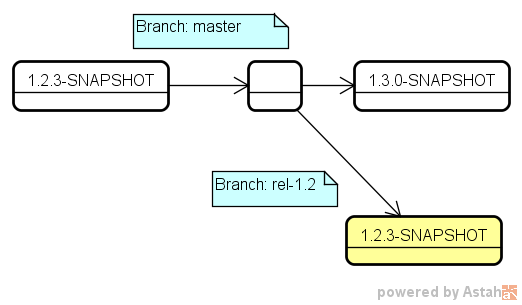
\includegraphics[width=0.7\linewidth]{img/branching_otojr_01}
	\caption[Branching de Release]{Cria{\c c}{\~a}o do branching de release}
	\label{fig:branchingrelease}
\end{figure}

\subsection{Detalhamento do Branch de Release}
\label{subsec:detalherelease}
Um questionamento comum em rela{\c c}{\~a}o à ramifica{\c c}{\~a}o de release {\'e} devido ao fato da mesma ser um branch e n{\~a}o um estado fechado (snapshot do SCM) marcado por uma tag. Ou seja, por que utilizar uma a{\c c}{\~a}o branch ao inv{\'e}s de uma a{\c c}{\~a}o tag?

Apesar de necess{\'a}rio considerar que no ponto de cria{\c c}{\~a}o do branch da release, o c{\'o}digo j{\'a} tenha passado por todo o ciclo de testes (unidade, regress{\~a}o, aceita{\c c}{\~a}o, etc), {\'e} imposs{\'i}vel afirmar que o produto a ser lan{\c c}ado est{\'a} livre de defeitos. Da{\'i} o motivo da exist{\^e}ncia do branch. Este branch {\'e} usado para corre{\c c}{\~a}o de defeitos da release at{\'e} a "lapida{\c c}{\~a}o" da vers{\~a}o final que ser{\'a} entregue ao cliente. 

O mais importante que devemos frisar {\'e} que neste branch est{\'a} proibido adicionar novas funcionalidades para que n{\~a}o ocorra uma regress{\~a}o de estabilidade no projeto. Neste branch, trabalha-se uma equipe dedicada somente a corre{\c c}{\~a}o de defeitos. Este ciclo de corre{\c c}{\~a}o de defeitos pode ocorrer em v{\'a}rias mini-itera{\c c}ões onde que cada itera{\c c}{\~a}o seja gerada uma nova vers{\~a}o de corre{\c c}{\~a}o neste mesmo branch. Cada vers{\~a}o nova de corre{\c c}{\~a}o deve ser reintegrada novamente ao branch master para que os desenvolvedores  recebam estas corre{\c c}ões e o branch principal se mantenha o mais est{\'a}vel poss{\'i}vel. 

As itera{\c c}ões de corre{\c c}{\~a}o ocorrem at{\'e} que a release esteja em um n{\'i}vel de qualidade acordada e aceitada pelo cliente. Neste momento ent{\~a}o, uma vers{\~a}o de produ{\c c}{\~a}o (n{\~a}o sufixada) deve ser constru{\'i}da, documentada e entregue ao cliente. Opcionalmente pode-se utilizar uma tag para marcar a vers{\~a}o que foi entregue. 

Por exemplo: no projeto FrameworkTeste, vers{\~a}o 1.2.3-SNAPSHOT, {\'e} criado o branch de release rel-1.2 onde uma determinada equipe trabalhar{\'a} com as corre{\c c}ões de defeitos. Neste branch, a cada conjunto de defeitos corrigidos, s{\~a}o gerados novas versões 1.2.4, 1.2.5, 1.2.6, at{\'e} a qualidade aceitada. Neste momento ent{\~a}o, digamos que a vers{\~a}o 1.2.6 est{\'a} apta a ser entregue ao cliente. Esta vers{\~a}o deve ser documentada como vers{\~a}o entregue e opcionalmente podemos marcar como uma tag v1.2.6-Final este ponto da release como mostrado na figura \ref{fig:finalrelease}.

\begin{figure}[h!]
	\centering
	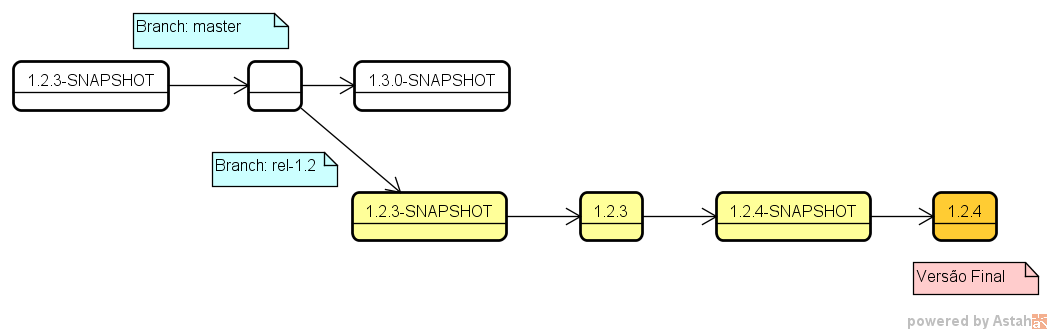
\includegraphics[width=0.7\linewidth]{img/branching_otojr_02}
	\caption[Cria{\c c}{\~a}o da vers{\~a}o final]{Cria{\c c}{\~a}o da vers{\~a}o final do produto a partir do branch da release.}
	\label{fig:finalrelease}
\end{figure}

\subsection{Hotfixes}
\label{subsec:hotfixes}
Ocasionalmente, uma vers{\~a}o entregue ao cliente pode apresentar algum defeito. N{\~a}o {\'e} desej{\'a}vel, mas tal situa{\c c}{\~a}o n{\~a}o {\'e} imposs{\'i}vel. Neste caso, {\'e} necess{\'a}rio que ocorra um Hotfix na vers{\~a}o final entregue. A forma de tratar Hotfixes neste modelo de trabalho proposto ocorre naturalmente no branch de release. É feita mais uma itera{\c c}{\~a}o de corre{\c c}{\~a}o no branch de release e gerada uma nova vers{\~a}o documentada (opcionalmente marcada com tag) como entregue. Pode ser visto na figura \ref{fig:hotfix}

\begin{figure}[h!]
	\centering
	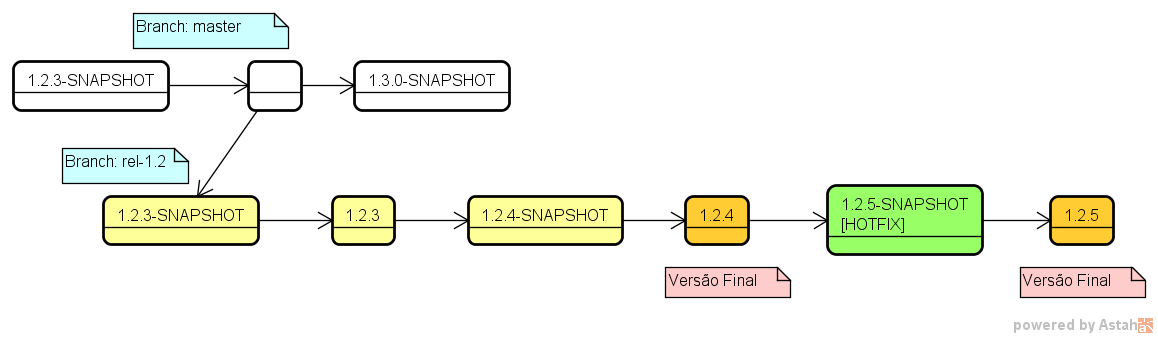
\includegraphics[width=0.7\linewidth]{img/branching_otojr_03}
	\caption[Hotfix na vers{\~a}o final]{Aplica{\c c}{\~a}o de um Hotfix na vers{\~a}o final do produto.}
	\label{fig:hotfix}
\end{figure}